% !TeX spellcheck = ca
\documentclass{article}
\usepackage[utf8]{inputenc}
\usepackage{graphicx}
\usepackage{tikz}
\usepackage{listings}
\usepackage{float}
\usepackage{amsmath}
\usetikzlibrary{positioning,fit,calc,arrows.meta, shapes}
\graphicspath{ {images/} }

%Tot això hauria d'anar en un pkg, però no sé com és fa

\newcommand*{\assignatura}[1]{\gdef\1assignatura{#1}}
\newcommand*{\grup}[1]{\gdef\3grup{#1}}
\newcommand*{\professorat}[1]{\gdef\4professorat{#1}}
\renewcommand{\title}[1]{\gdef\5title{#1}}
\renewcommand{\author}[1]{\gdef\6author{#1}}
\renewcommand{\date}[1]{\gdef\7date{#1}}
\renewcommand{\contentsname}{Índex}
\renewcommand{\maketitle}{ %fa el maketitle de nou
	\begin{titlepage}
		\raggedright{UNIVERSITAT DE LLEIDA \\
			Escola Politècnica Superior \\
			Grau en Enginyeria Informàtica\\
			\1assignatura\\}
		\vspace{5cm}
		\centering\huge{\5title \\}
		\vspace{3cm}
		\large{\6author} \\
		\normalsize{\3grup}
		\vfill
		Professorat : \4professorat \\
		Data : \7date
\end{titlepage}}
%Emplenar a partir d'aquí per a fer el títol : no se com es fa el package
%S'han de renombrar totes, inclús date, si un camp es deixa en blanc no apareix

\renewcommand{\figurename}{Figura}
\renewcommand{\tablename}{Taula}
\title{Práctica 4}
\author{Joaquim Picó Mora, Ian Palacín Aliana}
\date{20 de Desembre 2019}
\assignatura{Sistemes Concurrents i Paral·lels}
\professorat{F. Cores}
\grup{PraLab1}

%Comença el document
\begin{document}
	\maketitle
	\thispagestyle{empty}
	
	\newpage
	\pagenumbering{roman}
	\tableofcontents
	\newpage
	\pagenumbering{arabic}
	


% Petita estimació de si el sistema serà útil per l’empresa i és factible de ser desenvolupat 
% sota les restriccions existents, a fi de determinar si es tira endavant, o bé val la pena invertir 
% en un estudi de viabilitat més profund i seriós
%TODO: @horno Fes aquesta part

%. Domini  (NO es demana)
%Glossari de termes del domini

\section{Introducción}

En este documento se compara la eficiencia en tiempo que supone ejecutar la aplicación Indexing de forma concurrente i secuencial respecto de forma concurrente sincronizada.
\\\\
Los datos que se utilizaran para hacer el estudio saldrán de ejecutar de forma secuencial y concurrente el mismo ejemplo, calculando así el tiempo en que tarda en realizarse cada una de las ejecuciones. Este tiempo será el que luego se usará para comparar y sacar conclusiones.\\
De mismo modo se ejecutará varias veces el programa con distinto número de hilos de ejecución y se procederá a la comparación de los resultados.

\section{Gráfica}
Intel Core i5 7Gen QuadCore.
\begin{figure}[hbt!]
  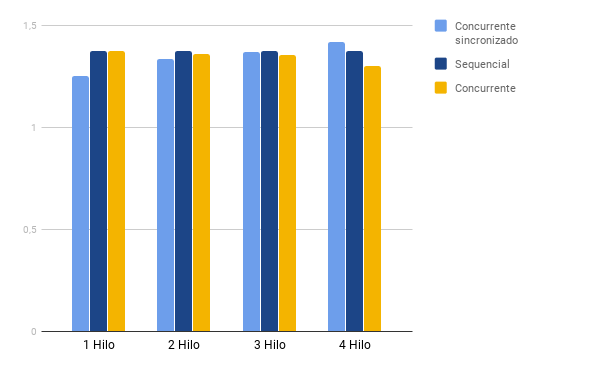
\includegraphics[width=\linewidth]{chart.png}
  \caption{Concurrente vs Sequencial vs Concurrente Sincronizado}
  \label{fig:convsseq}
\end{figure}
\newpage
\section{Concurrente vs Sequencial vs Concurrente Sincronizado}
En la anterior practica ya vimos que en general la versión concurrente tardaba más o menos lo mismo que la secuencial. Esto se producía debido a un cuello de botella cuando juntábamos los diferentes hashs generados en cada uno de los hilos. Esta vez, nos fijamos en que los tiempos también se asemejan bastante. Esto es debido a la sincronización que realizamos al añadir las claves al Mapa, cosa que hace que el tiempo al final termine siendo similar. Así pues, por el mismo precio hemos adquirido un programa plenamente Thread-Safe.

\section{Diferencias entre multiples hilos}
Como se ve en la gráfica la tendencia en el caso de la versión concurrente sincronizada es ligeramente ascendente. Esto quizás se deba a que contra más hilos más dependencias se generan, y más sincronizaciones tiene que hacer el programa.

\section{Diseño de la Solución}
Las dependencias que se han tratado son las siguientes:\\\\
-Introducción de llaves en el mismo HAshMap por parte de todos los threads. Para solucionar esta dependencia, se ha implementado un ReentrantLock que permite bloquear el mapa mientras se está escribiendo desde un hilo. En cuanto este termina, se libera el HashMap y otro hilo puede empezar a escribir en él.\\\\
Estadísticas Globales: Para la su realización se ha creado un objeto Stadistics desde el cual vamos a poder actualizar por medio de métodos los valores del objeto para así obtener las estadísticas. Para hacerlo de forma sincronizada se ha añadido la etiqueta syncronized en todos los métodos de la clase que modificaban un valor del objeto.\\\\
Estadísticas Locales: A la hora de imprimir las estadísticas locales de cada uno de los threads, se podía producir un fallo de sincronización con la E/S. Para evitarlo se ha utilizado el mismo método que con el mapa de llaves, un Reentrant Lock creado en el padre i utilizado en los hilos hijos para asegurar su correcta sincronización.\\\\
-Join Threads: Para implementar el join de los hilos se han utilizado un Semáforo. Este contiene el mismo número de permisos que de threads con los que se ejecuta nuestro programa. De esta forma en crear un thread se adquiere uno de los permisos y hasta que este no se termina no se libera. De mientras el hilo padre quedara bloqueado intentando adquirir los recursos con tantos permisos como threads con los que se ejecuta nuestro programa. De esta forma hasta que los threads no terminan su ejecución el padre no podrá continuar con la suya.

\end{document}

